\chapter{Introdução}

Adicionar motivação pelo tema - Por que resolver um problema ligado aos portadores de necessidades? (Obs - não é problematizar)

\section{O Problema}

	O desenvolvimento da opção mais básica de mobilidade para portadores de mobilidade reduzida, a cadeira de rodas, vem tornando-se cada vez mais estagnada. Mesmo com a adaptação do modelo clássico para modelos motorizados, não há, fora isso, muitas outras opções de mercado a fim de valorizar o conforto e facilitar a vida do usuário e seus familiares. Atualmente, a oferta de cadeira de rodas motorizadas com tecnologias semelhantes torna-se cada vez mais comum em um cenário onde um alto número de pessoas continua a optar por modelos clássicos devido aos altos custos dos modelos presentes no mercado internacional. A falta de opções com novas funcionalidades no mercado e o alto custo das soluções já existentes tornam o acesso a essas novidades cada vez mais restrito.\\
	
	Além disso, a ausência de um familiar ou cuidador em certos momentos do dia dificulta o monitoramento de atividades motoras ou necessidades do usuário. Com isso em foco, o monitoramento remoto contínuo do usuário poderia aumentar ainda mais sua liberdade em um ambiente doméstico e, ainda assim, manter familiares e cuidadores atentos a sinais e alertas e evitando possíveis acidentes e situações fora do cotidiano.\\
	
	O problema, juntamente às suas causas, são representados em um diagrama de Causa e Efeito, ou fishbone, conforme Figura \ref{fishbone}.
	
	\begin{figure}[h]
	\centering
	\label{fishbone}
		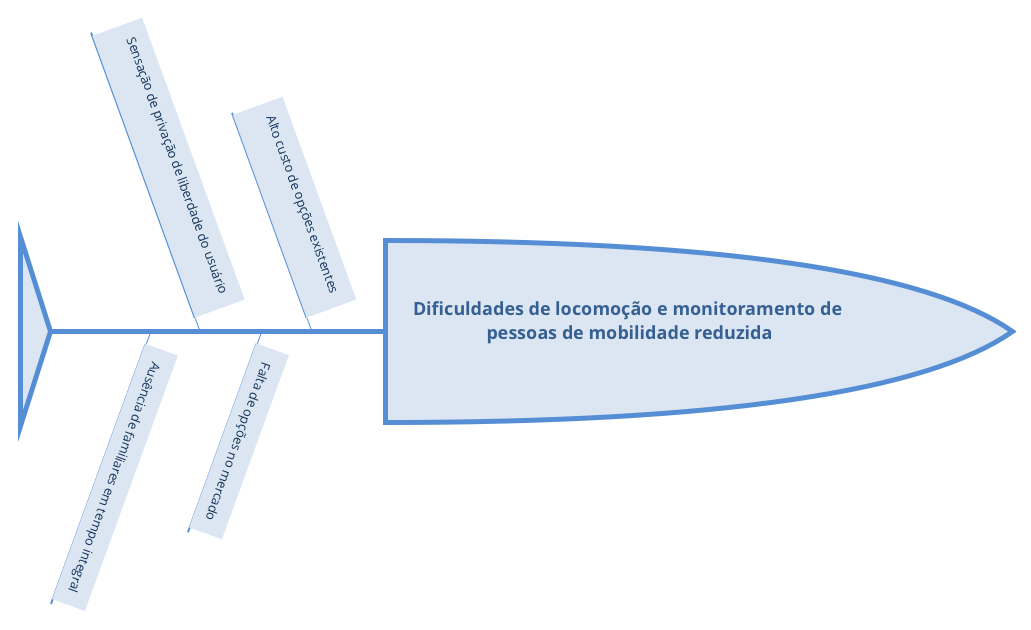
\includegraphics[keepaspectratio=true,scale=0.3]{figuras/fishbone.png}
	\caption{Diagrama de causa e efeito (\textit{fishbone}) para mapeamento do problema.}
\end{figure}


\section{Estado da Arte}

Fazer um levantamento das soluções atuais em volta do tema.

\section{Objetivos}

\subsection{Geral}

\subsection{Específicos}

\section{Proposta de Solução}

Fazer uma proposta de sistema EM ALTO NÍVEL sobre o problema, e porque essa solução é melhor que as mencionadas na seção anterior.

\section{Escopo}

O que a solução deverá abranger e não abranger.
